\documentclass[11pt,notes=hide,aspectratio=169,mathserif]{beamer}

% PACKAGES
\usepackage{graphics}  % Support for images/figures
\usepackage{graphicx}  % Includes the \resizebox command
\usepackage{url}	   % Includes \urldef and \url commands
\usepackage{natbib}
\usepackage{bibentry}  % Includes the \nobibliography command
\usepackage{verbatim}  %Supports comments
\usepackage{booktabs} %Supports \toprule, \bottomrule, etc in tables
\usepackage{etoolbox}  %Supports toggle commands
\usepackage{datetime}
\usepackage{bm}	%Supports bold math \bm

% PACKAGES (that should already be included by your LyX document settings)
\usepackage{amsfonts}  % Lots of stuff, including \mathbb 
\usepackage{amsmath}   % Standard math package
\usepackage{amsthm}    % Includes the comment functions

% CUSTOM DEFINITIONS
\def\newblock{} %Get beamer to cooperate with BibTeX
\linespread{1.2}

% IDENTIFYING INFORMATION
\title[Aldermanic Privilege]{Does Local Control Affect Density? Evidence from Chicago's Aldermanic Privilege}
\author[Jacob Herbstman]{Jacob Herbstman (University of Chicago)}
\date{\monthname[\the\month] \the\year}

% THEMATIC OPTIONS
\setbeamercovered{transparent}
\usetheme{metropolis}
\usecolortheme{default}
\beamertemplatenavigationsymbolsempty
\setbeamertemplate{footline}[frame number]{}

% BACKUP SLIDE NUMBERING
\usepackage{appendixnumberbeamer}

%SETTINGS
\newtoggle{shortertalk}
\togglefalse{shortertalk}

\begin{document}

%---------------------------------------------------------------------
\begin{frame}[plain]
\titlepage
\note{
	\begin{itemize}
	\end{itemize}
}
\end{frame}
%---------------------------------------------------------------------
\section{Motivation}

\begin{frame}
	\begin{itemize}
		\item Chicago alderman have substantial power to shape local land use and development decisions
		\item It has received increased scrutiny in recent years, from both local politicians and the federal government
	\end{itemize}
\end{frame}


\begin{frame}
    \begin{minipage}{0.5\textwidth}
        \begin{figure}
            \centering
            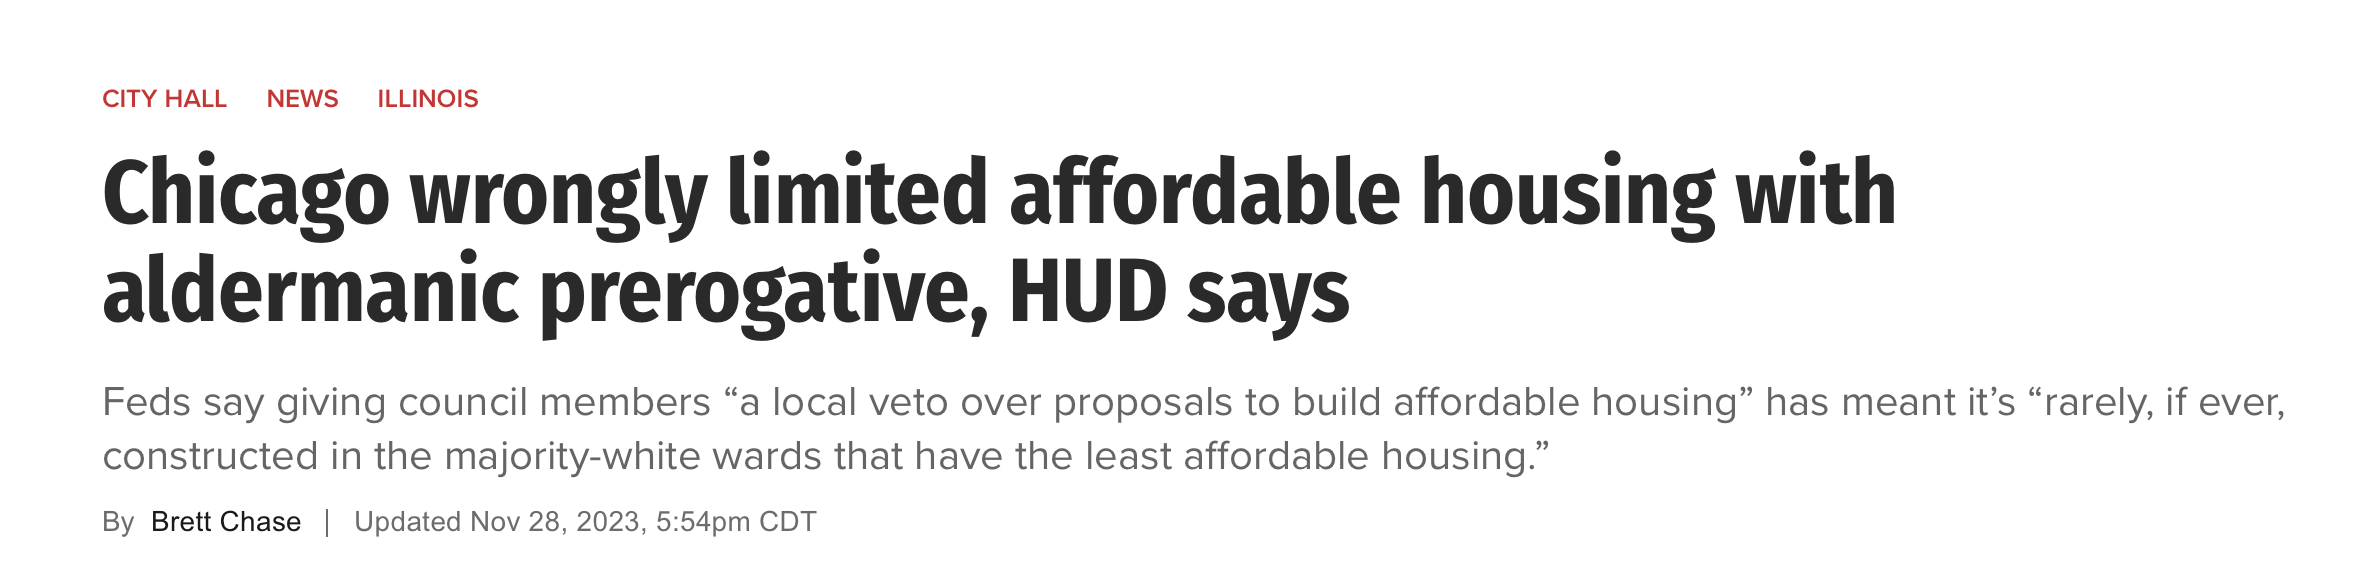
\includegraphics[width=\textwidth]{images/hud_report_headline.png}
			\vspace{20pt}
			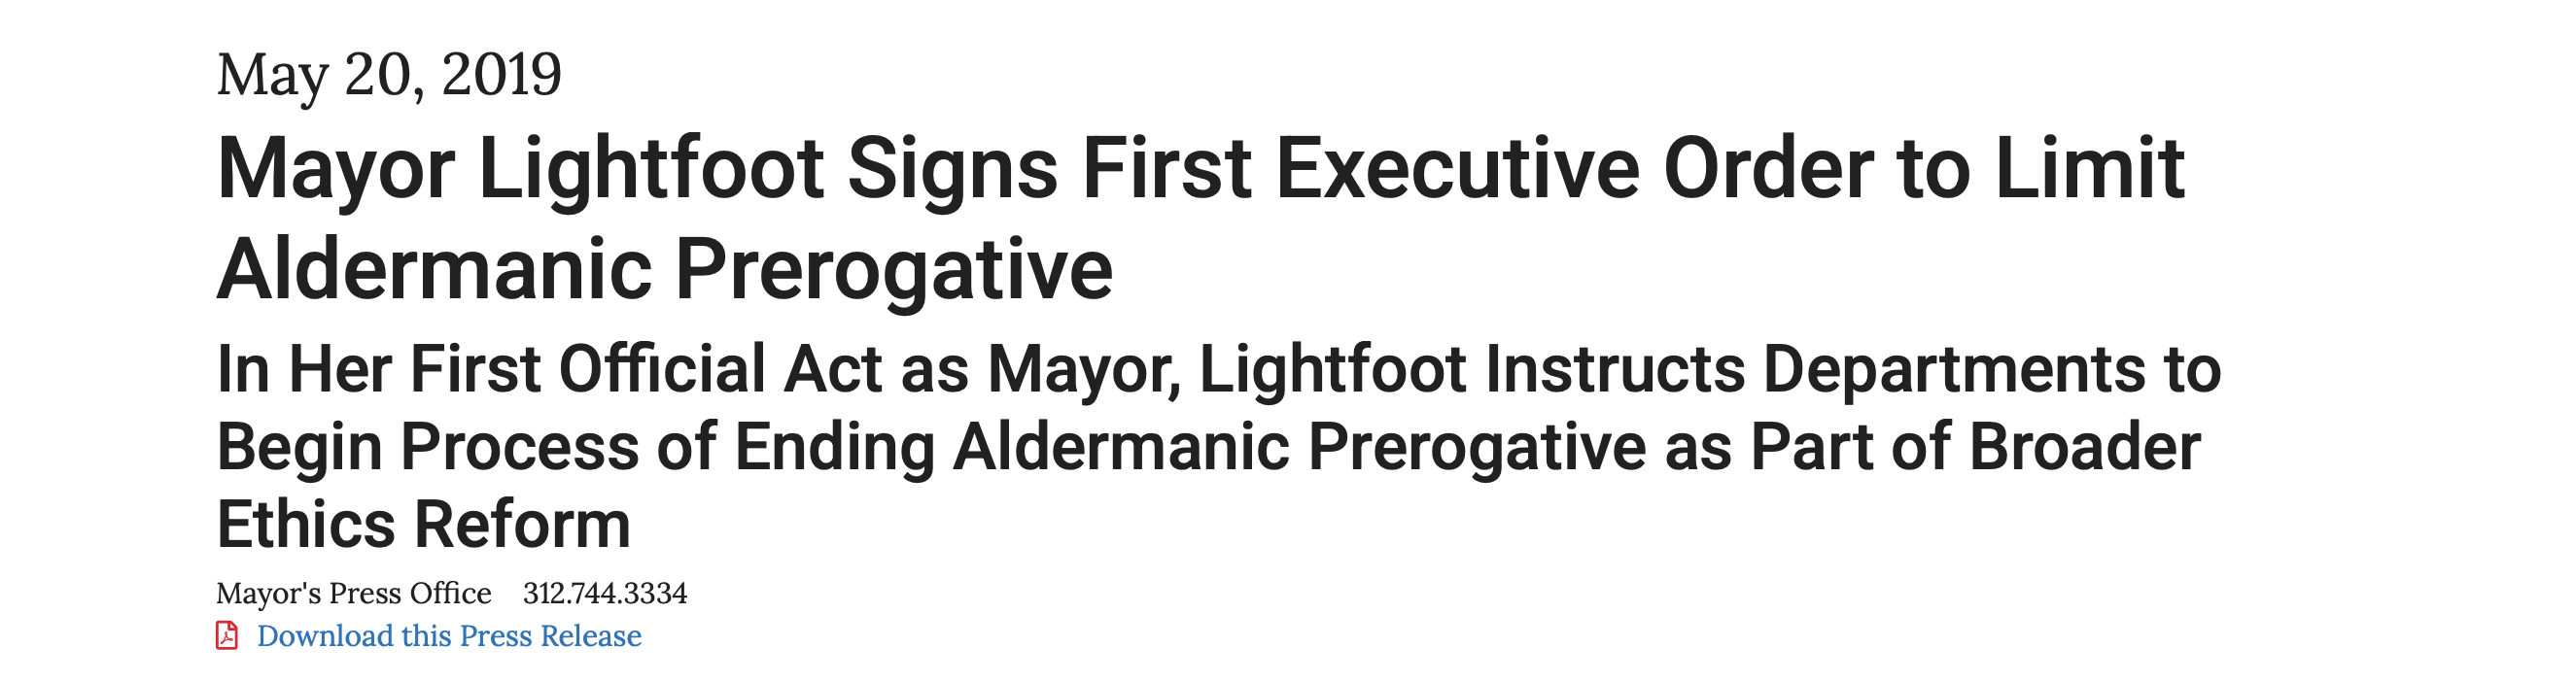
\includegraphics[width=\textwidth]{images/lightfoot_order.png}
        \end{figure}
        \end{minipage}
        \hfill
        \begin{minipage}{0.48\textwidth}
        \begin{figure}
            \centering
            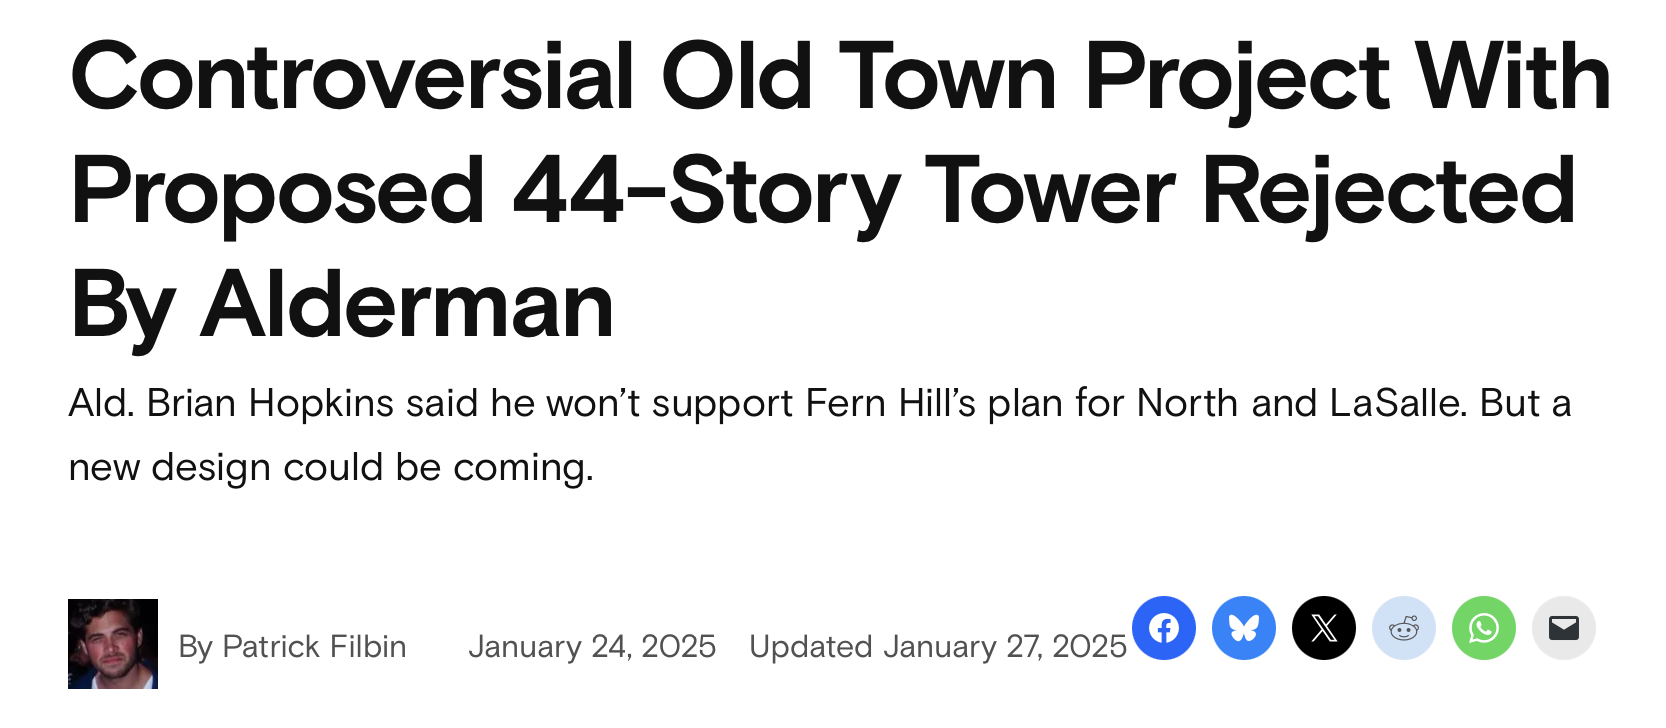
\includegraphics[width=\textwidth]{images/old_town_towers.png}
			\vspace{20pt}
			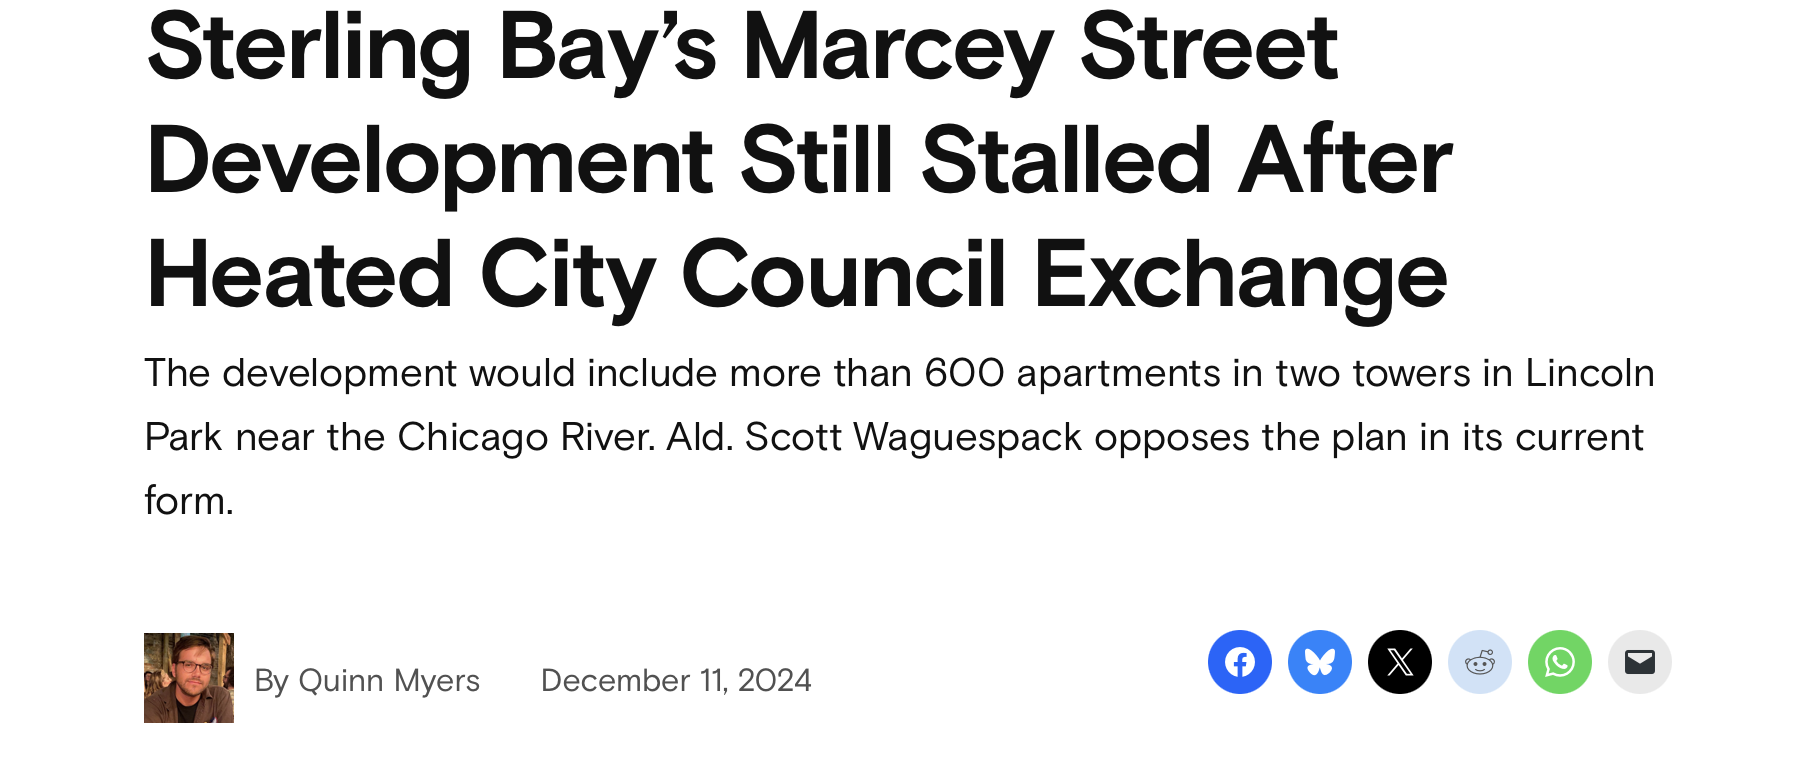
\includegraphics[width=\textwidth]{images/sterling_bay_fight.png}
        \end{figure}
        \end{minipage}
\end{frame}
\begin{frame}
	\begin{itemize}
        \item \textbf{Decentralized Urban Governance}
        \begin{itemize}
            \item {\scriptsize \cite{levine_effects_1999, khan_decentralized_2021,brueckner_bunching_2024, 
            mast_warding_2024,bordeu_commuting_2025}}
        \end{itemize}
        \vspace{1em} 

        \item \textbf{Incumbent Residents' Influence on Development}
        \begin{itemize}
            \item \scriptsize{\cite{fischel_homevoter_2009, rossihansberg_housing_2010, ortalo-magne_political_2014,freemark_upzoning_2020}}
        \end{itemize}
        \vspace{1em}
    
        \item \textbf{Spatial Regression Discontinuity Designs}
        \begin{itemize}
            \item \scriptsize{\cite{black_better_1999,bayer_unified_2007,turner_land_2014,monarrez_dividing_2023}}
        \end{itemize}
        \vspace{1em}
    
    \end{itemize}
\end{frame}

\begin{frame}
    \frametitle{Data Sources}
	\begin{itemize}
        % Item 1: Appears on slide 1 and stays visible.
        \item<1-> \textbf{Attom Data}
        % Details for item 1: Only appear on slide 1.
        \only<1>{
            \begin{itemize} 
                \item I use parcel-level data from Attom to create a sample of all new residential developments in Chicago from 2006-2023
                \item Contains exact geocoded location, lot size, square footage, number of units, and many other characteristics
                \item My final analysis sample contains $\approx 15,000$ unique developments
            \end{itemize}
        }
        \vspace{1em} 

        % Item 2: Appears on slide 2 and stays visible.
        \item<2-> \textbf{Chicago Building Permits Data}
        % Details for item 2: Only appear on slide 2.
        \only<2>{
            \begin{itemize}
                \item To create alderman fixed effects for the RD design, I use publicly-available permit data from the City of Chicago
                \item Includes over $800,000$ permits from 2006-2023, with exact geocoded location and permit type
                \item I also obtain ward shapefiles from the City of Chicago Data Portal
            \end{itemize}
        }
        \vspace{1em}
    
        % Item 3: Appears on slide 3 and stays visible.
        \item<3-> \textbf{Demographic Data}
        % Details for item 3: Only appear on slide 3.
        \only<3>{
            \begin{itemize}
                \item I obtain demographic variables at the block-group level from the American Community Survey (ACS)
                \item Used to create ward-level control variables for alderman fixed-effects regressions
                \item Include median income, population density, homeownership rate, and racial composition of each ward
            \end{itemize}
        }
        % No vspace needed after the last item, but you can add it if you want.
    \end{itemize}
\end{frame}







\begin{frame}
    \frametitle{Empirical Strategy: Alderman Fixed Effects} 
        % Details for item 1: Only appear on slide 1.
        \only<1>{
            \begin{itemize} 
                \item For my stacked RD design, I need to "sign" each ward border to create a negative and positive side
                \item To do so, I use the permit dataset to create a measure of alderman "strictness" by running the following regressions at the montly level: 
                \[
                \begin{aligned}
                    Y_{it} = \beta_0 + \sum_{j=1}^{N-1} \delta_j \cdot \text{Alderman}_j + \mathbf{X}{it}'\boldsymbol{\gamma} + \lambda_t + \epsilon_{it}
                \end{aligned}
                \]
                \item $Y_{it}$ contains 4 outcome variables: (1) log permits issued, (2) permit approval rate, (3) log average permit processing time, and (4) log average total fee for each project
                \item $\delta_j$ are the $N-1$ alderman fixed effects, all referenced to Andre Vasquez (40th Ward), but this is arbitrary
            \end{itemize}
        }
\end{frame}

\begin{frame}
    \frametitle{Empirical Strategy: Alderman Fixed Effects} 
        % Details for item 1: Only appear on slide 1.
        \only<1>{
            \begin{itemize} 
                \item Results are robust to a ward + month fixed effects, but lose a lot of power in the RD since many wards don't have any variation in representation
                \item I then take the first principal component of the 4 $\hat{\delta}_j$ estimates to create a single "strictness" score for each alderman
            \end{itemize}
        }
\end{frame}


\begin{frame}
   \frametitle{Results: Alderman Fixed Effects} 
       \begin{figure}
           \centering
           \includegraphics[width=\textwidth,height=0.82\textheight,keepaspectratio]{../tasks/create_alderman_strictness_scores/output/Month_FEs_final_strictness_index.pdf}
           \label{fig:alderman_effects}
       \end{figure}
\end{frame} 
%---------------------------------------------------------------------

%---------------------------------------------------------------------
\begin{frame}[plain]
    \begin{center}{\LARGE Thank you}\end{center}
    \end{frame}
%---------------------------------------------------------------------

%---------------------------------------------------------------------
% A frame to display the bibliography
\begin{frame}[allowframebreaks]{}
    \bibliographystyle{aer}
    \bibliography{sections/aldermanic_privilege}
\end{frame}
%---------------------------------------------------------------------





%\beginbackup
\appendix
%\begin{frame}[plain]
  \begin{center}{\LARGE Appendix}\end{center}
  \end{frame}
%------------------
% APPENDIX PLOTS 
\begin{frame}[t,label=levels]
  \frametitle{Results: Floor Area Ratio (FAR)} 
  \begin{figure}
      \centering
      \includegraphics[width=\textwidth,height=0.75\textheight,keepaspectratio]{../tasks/spatial_rd/output/rd_plot_density_far_bw528_triangular.pdf}
      \label{fig:spatial_rd_lapu}
  \end{figure}
  \vfill\hfill \hyperlink{far-main}{\beamerreturnbutton{Back}}
\end{frame}

\begin{frame}[t,label=lapu]
    \frametitle{Results: Log(Lot Area Per Unit (LAPU))} 
    \begin{figure}
        \centering
        \includegraphics[width=\textwidth,height=0.75\textheight,keepaspectratio]{../tasks/spatial_rd/output/rd_plot_log_density_lapu_bw528_triangular.pdf}
        \label{fig:spatial_rd_lapu}
    \end{figure}
    \vfill\hfill \hyperlink{far-main}{\beamerreturnbutton{Back}}
  \end{frame}

  \begin{frame}[t,label=bcr]
    \frametitle{Results: Log(Building Coverage Ratio (BCR))} 
    \begin{figure}
        \centering
        \includegraphics[width=\textwidth,height=0.75\textheight,keepaspectratio]{../tasks/spatial_rd/output/rd_plot_log_density_bcr_bw528_triangular.pdf}
        \label{fig:spatial_rd_lapu}
    \end{figure}
    \vfill\hfill \hyperlink{far-main}{\beamerreturnbutton{Back}}
  \end{frame}

  \begin{frame}[t,label=lps]
    \frametitle{Results: Log(Lot Size Per Story (LPS))} 
    \begin{figure}
        \centering
        \includegraphics[width=\textwidth,height=0.75\textheight,keepaspectratio]{../tasks/spatial_rd/output/rd_plot_log_density_lps_bw528_triangular.pdf}
        \label{fig:spatial_rd_lapu}
    \end{figure}
    \vfill\hfill \hyperlink{far-main}{\beamerreturnbutton{Back}}
  \end{frame}



   % APPENDIX TABLES 


  \begin{frame}[t,label=levels_FAR_table]{Results: Floor Area Ratio (FAR)}
    \centering
    \scriptsize{\input{../tasks/border_pair_FE_regressions/output/fe_table_density_far.tex}}
    \vfill\hfill \hyperlink{main_FAR_table}{\beamerreturnbutton{Back}}
  \end{frame}

  \begin{frame}[t,label=lapu_table]{Results: Log(Lot Area Per Unit (LAPU))}
    \centering
    \scriptsize{\input{../tasks/border_pair_FE_regressions/output/fe_table_log_density_lapu.tex}}
    \vfill\hfill \hyperlink{main_FAR_table}{\beamerreturnbutton{Back}}
  \end{frame}

  \begin{frame}[t,label=bcr_table]{Results: Log(Building Coverage Ratio (BCR))}
    \centering
    \scriptsize{\input{../tasks/border_pair_FE_regressions/output/fe_table_log_density_bcr.tex}}
    \vfill\hfill \hyperlink{main_FAR_table}{\beamerreturnbutton{Back}}
  \end{frame}

  \begin{frame}[t,label=lps_table]{Results: Log(Lot Size Per Story (LPS))}
    \centering
    \scriptsize{\input{../tasks/border_pair_FE_regressions/output/fe_table_log_density_lps.tex}}
    \vfill\hfill \hyperlink{main_FAR_table}{\beamerreturnbutton{Back}}
  \end{frame}




%\bibliographystyle{../bib/aeanobold}
%\nobibliography{../bib/bib.bib}
%\backupend


\end{document}